\documentclass[10pt]{standalone}

\usepackage{tikz}
\usepackage[cmex10]{amsmath}
\usepackage{xfrac}
\usepackage{xcolor}

\usetikzlibrary{calc}
\usetikzlibrary{arrows}
\usetikzlibrary{arrows.meta}
\usetikzlibrary{positioning}
\usetikzlibrary{decorations.text}
\usetikzlibrary{decorations.pathmorphing}

\definecolor{bluish}{RGB}{101,161,216}
% \definecolor{colorA}{HTML}{FF48CF} % magenta
% \definecolor{colorB}{HTML}{8770FE} % purple
% \definecolor{colorC}{HTML}{1BA1EA} % blue
\definecolor{seagreen}{HTML}{14B57F}
% \definecolor{colorE}{HTML}{3EAA0D} % green
% \definecolor{colorF}{HTML}{C38D09} % orange
% \definecolor{colorG}{HTML}{F5615C} % red

\newcommand{\paren}[1]{\left(#1\right)}

\begin{document}

	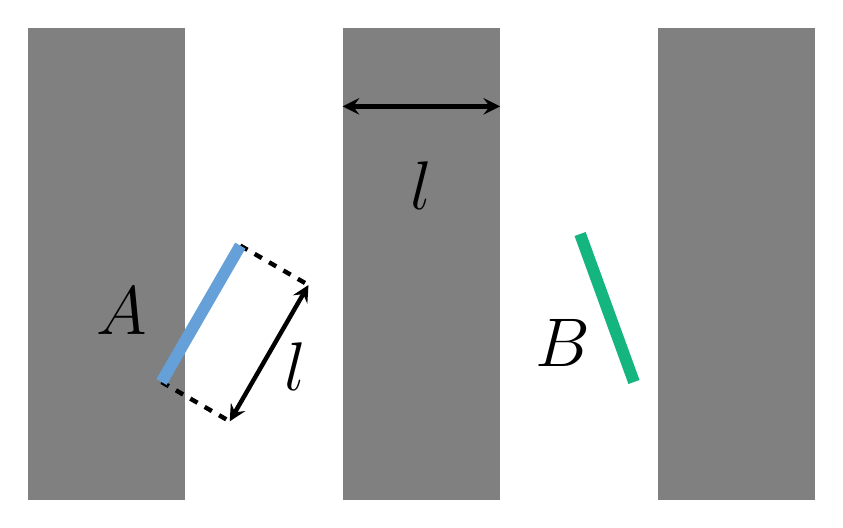
\begin{tikzpicture}[x=2cm, y=2cm]
		\fill[gray] (0,0) rectangle ++(1,3);
		\fill[gray] (2,0) rectangle ++(1,3);
		\fill[gray] (4,0) rectangle ++(1,3);

		\coordinate (A) at (0.85,0.75);
		\draw[black, ultra thick, dashed] (A) -- ++(330:0.5);
		\draw[black, ultra thick, dashed] ($(A)+(60:1)$) -- ++(330:0.5);
		\draw[black, >=stealth, <->, ultra thick] ($(A)+(330:0.5)$) -- ($(A)+(60:1)+(330:0.5)$);
		\draw[bluish, line width=0.15cm] (A) -- ++(60:1);
		\draw[draw=none, fill=none] (1.7,0.85) node {\Huge $l$};
		\draw (0.6,1.2) node {\Huge $A$};

		\coordinate (B) at (3.85,0.75);
		\draw[seagreen, line width=0.15cm] (B) -- ++(110:1);
		\draw (3.4,1) node {\Huge $B$};

		\draw[black, >=stealth, <->, ultra thick] (2,2.5) -- (3,2.5);
		\draw (2.5,2) node {\Huge $l$};
	\end{tikzpicture}

\end{document}